\newpage
\section{Ethernet 2 (Ethernet Systeme)}

\subsection{Virtuelle LANs}

\paragraph{Trunk-Links} Trunk Links sind Teil von mehreren VLANs. Auf den Trunk Links müssen Frames der verschiedenen VLANs eindeutig gekennzeichnet werden!

\paragraph{VLAN-Tag} Erweiterung des Ethernet Headers durch einen
VLAN-Tag.
Die maximalen Nutzdatenlänge bleibt erhalten,
der Ethernet Frame wird 4 Bytes länger
{
\begin{itemize}[noitemsep]
    \item Type 0x8100 $\to$ getaggtes Frame
    \item Priority Code Point ermöglicht die Priorisierung gewisser Applikationen
    \item Discard Eligibility Indicator 0 → Frame wird bei Überlastsituationen zuerst verworfen
    \item VLAN Tagging erfolgt oft beim Eintritt / Austritt ins Netz
    \item  Für Endgeräte unsichtbar
\end{itemize}
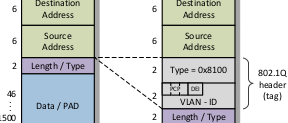
\includegraphics[scale=.75]{img/vlan.png}
\WhiteSpace
}

\subsection{Spanning Tree}

{\paragraph{Ziel:}  Alle Segmente in einer loop-freien Topologie verbinden.
    Beim Spanning-Tree werden von redundanten Pfaden alle ausser einer gesperrt. Im Fehlerfall wird falls möglich ein ausgefallener Port ersetzt.
    Der Algorithmus bestimmt eine Root-Bridge, von welcher aus dem Baum aufgespannt wird.}

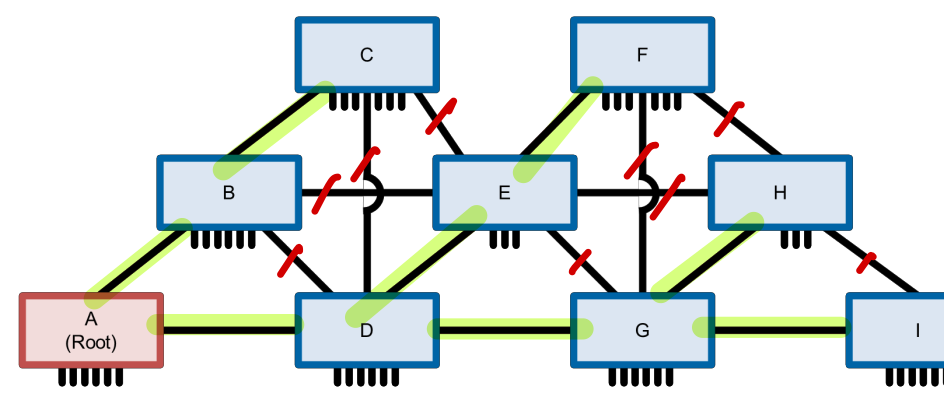
\includegraphics[scale=.275]{img/spanning_tree.png}

\subsection{Autonegotiation}


\paragraph{Ziel:}  Ermittlung der besten Betriebsart durch Austausch der
Leistungsmerkmale zweier Netzwerkkomponenten.


\subsection{Bridges}
{Bridges verfügen über einen Mechanismus zum Erlernen von Adressen. Eine Bridge hört den Verkehr von allen Ports ab und merkt sich die Sender-Adressen aus den
    empfangenen Frames in der sogenannten «Filtering Database».}
\paragraph{Filtering Database} beinhaltet für jede bekannte Mac-Adresse das Bridge-Port, über welches der zugehörige
Knoten erreichbar ist. Unbenutzte Einträge in der Filtering Database werden nach einer gewissen Zeit automatisch gelöscht

\subsection{Router}

\paragraph{Router}  sind Komponenten, die es erlauben Subnetze miteinander zu verbinden. Router haben eine ähnliche Funktion wie Bridges, allerdings arbeiten sie auf dem
Network Layer.
    {
        \begin{itemize}[noitemsep]
            \item Router empfangen nur Pakete, die direkt an sie adressiert sind.
            \item Die Weiterleitung erfolgt anhand der Network Layer Adresse.
            \item DBenutzen immer den optimalen Pfad.
            \item  Für Endgeräte unsichtbar
        \end{itemize}
    }

\paragraph{ Routing-Tabelle}
{
    \begin{itemize}[noitemsep]
        \item Sortiert nach der Länge der Netzmaske
        \item Von oben nach unten durchsucht
        \item Verglichen werden die Netzadressen
    \end{itemize}
}

\subsection{ARP (Address Resolution Protocol)}

\paragraph{Ziel:}  Ermittlung der MAC-Adresse zu einer IP-Adresse.

\subsection{ARP (Internet Protokoll Format (IP-Header))}
{Ein IP-Packet besteht aus einem Header (min. 20 Byte) und Nutzdaten.}
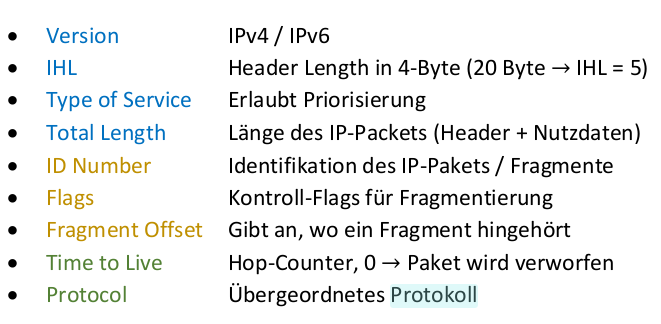
\includegraphics[scale=0.375]{img/ip-header-1.png}
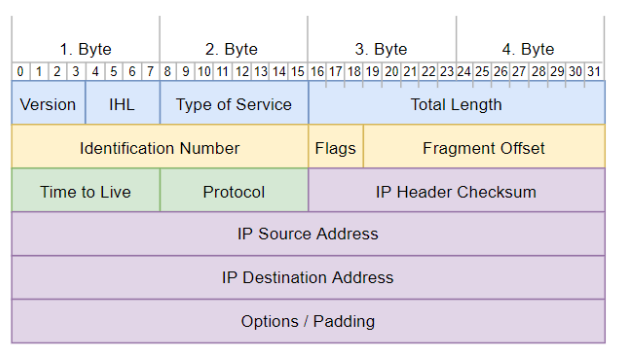
\includegraphics[scale=0.4125]{img/ip-header-2.png.png}
{Das unterliegende Netz limitiert die Grösse eines Pakets (Maximum Transfer Unit). Der Sender kennt die MTU der Netze nicht.}

\subsection{Fragmentierung}{
    Um über Netze mit verschiedenen Maximum Transfer Units (MTU) arbeiten zu können, unterstützt IP
    Fragmentierung und Reassembly.
    \begin{itemize}[noitemsep]
        \item Länge der Nutzdaten = Vielfaches von 8 Bytes
        \item Die Pakete haben die gleiche und grösstmögliche Länge
    \end{itemize}

    Jedes IP Fragment beinhaltet alle notwendigen Daten um den Endknoten zu erreichen (IP Header) und ein
    Vielfaches von 8 Bytes an Transportlayer-Daten (Ausnahme: letztes Fragment)
}

\subsection{Reassembly}{
    \begin{itemize}[noitemsep]
        \item 1. Zusammensetzen beim Zielhost
        \item 2. Letztes Fragment: MF = 0
    \end{itemize}}
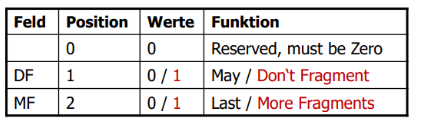
\includegraphics[scale=0.5]{img/fragment.png}

\subsection{Internet-Adressierung (IPv4)}{
    \begin{itemize}[noitemsep]
        \item Netzadresse $\to$ Tiefste Adresse im Subnetz
        \item Broadcast $\to$ Höchste Adresse im Subnetz
    \end{itemize}

    Beispiel im Anhang.

    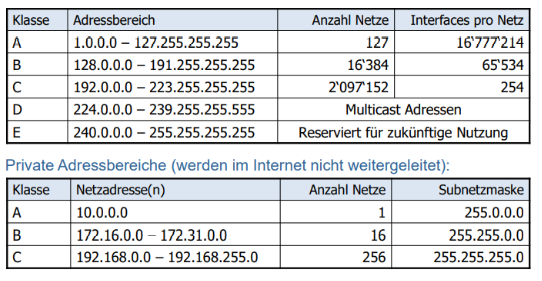
\includegraphics[scale=0.425]{img/netztklassen.png}


}
